\section{Robust Machine Learning}

\begin{frame}{Robust Machine Learning}
    思想:很多机器学习算法只要对输入数据进行微小的扰动,输出结果就完全错误了。希望能有一种方法能够让机器学习算法对输入数据的扰动具有一定的鲁棒性。

    几种方法:
    \begin{itemize}
        \item FGSM: 当学习率趋于无穷时,先更新再投影到正方体内结果大概率是顶点上。
        \item PGD: run gradient descent, and then project it back.
    \end{itemize}
    
    详见 Yang Yuan slides。
\end{frame}

\begin{frame}{Robust Features are Important}
    \begin{itemize}
        \item 左图实验发现,从原始既包含Robust Features也包含Non-Robust Features的数据集上只提取Robust Features部分,并在获得的新数据集Robust dataset上进行训练,
        可以得到类似的standard accuracy和robust accuracy(与在原始训练集上训练的结果相比)。
        \item 这说明模型可以只从Robust Features中学习,而不必须学习Non-Robust Features。
        \item Note: Robust Features 通常指人能看到的特征,因为人识别就是Robust的。
    \end{itemize}
    \begin{center}
        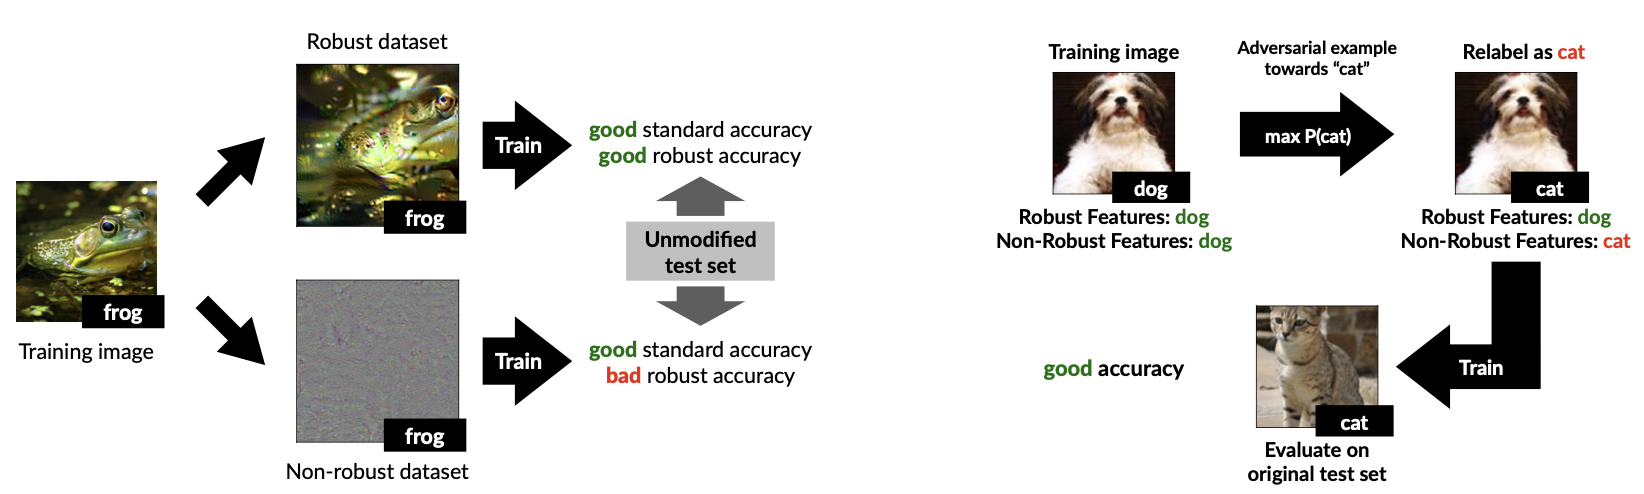
\includegraphics[width=0.8\textwidth]{assets/rml.png}
    \end{center}
\end{frame}

\begin{frame}{Non-Robust Features are also Important}
    \begin{itemize}
        \item 右图实验:通过调整Non-Robust Features 让其向某错误的标签$c_\text{wrong}$偏移,然后构建一个新的数据集,这个数据集标签是按照$c_\text{wrong}$来标记的,图像是原图像加上Non-Robust Features的偏移之后的图像。
        \item 由于 Robust Feature没有变化,人作为Robust Learner,仍然能够正确识别这些图像。
        \item 但实验结果表明,模型用这个新数据集训练,在原始test set上测试 accuracy 差不多不变,这说明模型也可以只从Non-Robust Features中学习。
    \end{itemize}
    \begin{center}
        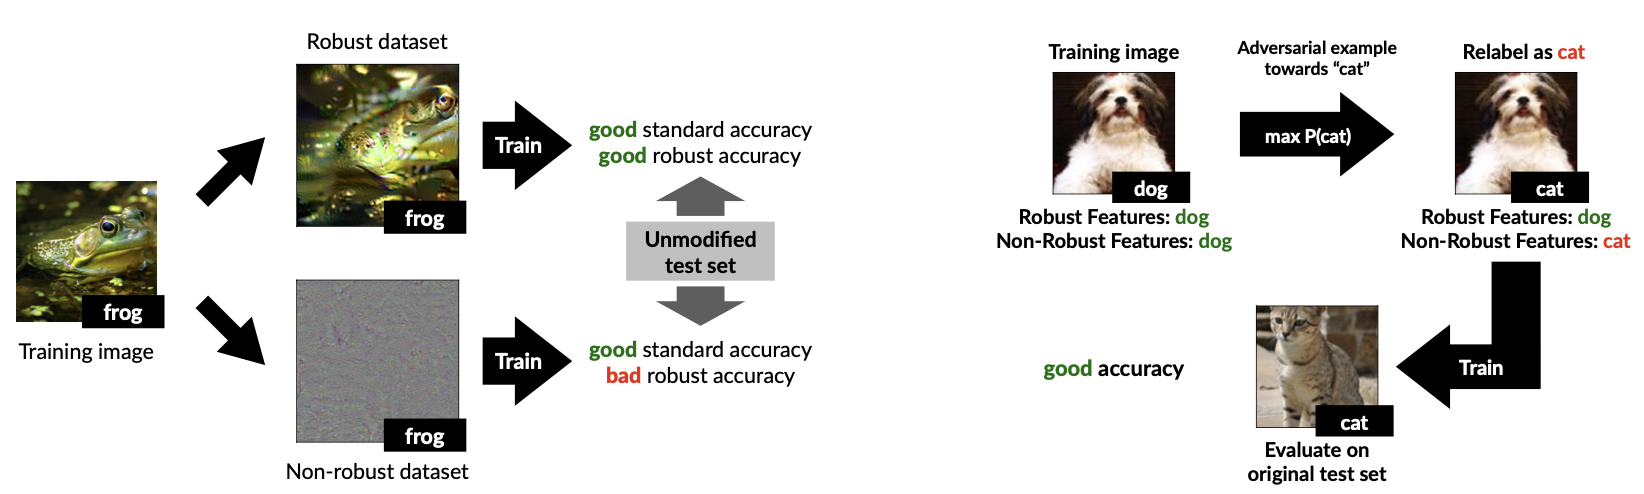
\includegraphics[width=0.8\textwidth]{assets/rml.png}
    \end{center}
\end{frame}

\begin{frame}[fragile]{Greedy Filling}
    \begin{itemize}
        \item 问题:已知一个分类器$f$,希望构建一个平滑分类器$g$,使预测更加robust。
        \item 自然想法:对单个输入$x$,不只考虑$f(x)$的值,还考虑$f(x')$的值,其中$x'$与$x$在输入空间中非常接近。
        \item 具体的:$g(x)$ 按照某概率分布函数$p(x')$(中心为$x$)加权,求不同标签$c$对应的$x'$占据的概率比例,概率比例最大的那个标签作为$g(x)$的预测结果。
        \[
            g(x) = \text{arg}\max_{c} \int_{x'} p(x') \mathbbm{1} [f(x') = c] \mathrm{d}x'
        \]
        \item Greedy Filling 算法用于计算对于给定输入点$x$和给定每个标签$c$对应的$\int_{x'} p(x') \mathbbm{1} [f(x') = c] \mathrm{d}x'$的值(即给定每种标签的概率直方图),在最坏情况下,$x$ 偏移多少就有可能让$g(x)$的预测结果发生变化。
        \item 以下为简单,只考虑二分类问题(只有两个 class $c_1$ 和 $c_2$)的Greedy Filling算法。
    \end{itemize}
\end{frame}

\begin{frame}[fragile]{Greedy Filling Example 1: Unit Ball}
    \begin{itemize}
        \item 将概率分布函数$p$取为单位球$B = \left\{x'\in \mathbb{R}^{d} | \left\| x' - x \right\| _2 \leqslant R \right\} $ 内的均匀分布
        \[
            p(x') = \begin{cases}
                \frac{1}{\text{Vol}(B)} & x' \in B \\
                0 & \text{otherwise}
            \end{cases}
        \]
        \item 目标:求$\delta$使$\left\| \delta \right\|_2 $最小,且$g(x+\delta)$能改变最大概率对应的class (二分类问题中就是两个class概率各为$50\%$)。
    \end{itemize}
\end{frame}

\begin{frame}[fragile]{Greedy Filling Example 1: Unit Ball}
    \begin{itemize}
        \item 目标:求$\delta$使$\left\| \delta \right\|_2 $最小,且$g(x+\delta)$能改变最大概率对应的class (二分类问题中就是两个class概率各为$50\%$)。
        \item 记$S_1 = \left\{ x'\in \mathbb{R}^{d} | \left\| x' - x \right\| _2 \leqslant R \right\} $, $S_2 = \left\{ x'\in \mathbb{R}^{d} | \left\| x' - x - \delta \right\| _2 \leqslant R \right\} $
        \item 不妨设$B$的体积为$1$,给定$x$点以及给定两个class $c_1$ 和 $c_2$在$x$点处概率占比为$80\%$ 和 $20\%$,按照 Greedy 的核心思想,为了让$g(x+\delta)$的预测结果发生尽量大的变化,
        \begin{itemize}
            \item 若 $\text{vol}(S_1-S_2) \geqslant 0.8$, 应将 $S_2-S_1$内全部假设为$c_2$类,由于有两个class $c_1$ 和 $c_2$在$x$点处概率占比为$80\%$ 和 $20\%$的约束,所以将 $S_1-S_2$内$0.8$体积假设为$c_1$类,其他$S_1$中体积假设为$c_2$类。
            \item 若 $\text{vol}(S_1-S_2) < 0.8$, 应将 $S_1-S_2$内全部假设为$c_1$类,$S_2-S_1$内全部为$c_2$类,$S_1 \hat S_2$ 内体积为$0.8 - \text{vol}(S_1-S_2)$ 填成 $c_1$, 其他填成 $c_2$。
        \end{itemize}
        据此可以求出$\left\| \delta \right\|_2 $的最小值。
    \end{itemize}
\end{frame}
    
\begin{frame}[fragile]{Greedy Filling Example 2: Gaussian Distribution}
    \begin{itemize}
        \item 将概率分布函数$p$取为 Gaussian Distribution
        \[
            p(x') = \frac{1}{(2\pi)^{d/2} \sigma^d} \exp\left( -\frac{1}{2\sigma^2} \left\| x' - x \right\|_2^2 \right)
        \]
        (作业中取$\sigma = 1$)
        \item 目标:求$\delta$使$\left\| \delta \right\|_2 $最小,且$g(x+\delta)$能改变最大概率对应的class。不妨假设$g(x) = c_1$。
        \item 按照 Greedy 的核心思想,为了让$g(x+\delta)$的预测结果发生尽量大的变化,应该先从 $p(x' - x - \delta)/p(x' - x)$ 最大的 $x'$ 处开始设成 $c_2$,因为先从这里开始选取 $c_2$ 可以让$g(x+\delta)$中$c_2$的成分相较$g(x)$中$c_2$的成分增加最多。
        \item 再由高斯分布的特性,$p(x' - x - \delta)/p(x' - x)$ 的等值线是超平面,退化为一维问题,$\left\| \delta \right\|_2 $的最小值容易求解。(剩下的步骤参考习题课)
    \end{itemize}
\end{frame}

